% !TEX TS-program = xelatex
%
% Created by Gerson Sunyé on 2016-12-14.
% Copyright (c) 2016 .
\documentclass[a4paper,11pt]{memoir}
\usepackage[]{xsim}
\usepackage[utf8]{inputenc}
\usepackage{lmodern}
\usepackage{listings,multicol}
\usepackage{hyperref}
\usepackage{graphicx}
\usepackage[svgnames]{xcolor}
\usepackage{polyglossia}
\setdefaultlanguage{english}
\usepackage{pdfpages}
\usepackage{typehtml}
\usepackage{lscape}
\usepackage[french,boxed,lined]{algorithm2e}
\usepackage{amsmath}
\usepackage{siunitx}
\xsimsetup{solution/print=false}
\usepackage{booktabs}
\usepackage{paralist}


\lstset{basicstyle=\tiny,
	keywordstyle=\bfseries,
	stringstyle=\ttfamily,
	showstringspaces=\false,
	frame=tb,
	commentstyle=\itshape\color{magenta},
	extendedchars=true,
	showtabs=false,
	tabsize=2,
	tab=$\mapsto$,
	numbers=left, 
	numberstyle=\tiny,
	sensitive,
	texcl,
	breaklines=true,
	literate={é}{e}{1} {à}{a}{1}
	}

\lstnewenvironment{java}{\lstset{language=Java,        
        flexiblecolumns,
		keywordstyle=\bfseries,
        sensitive, 
		texcl
        }}{}

\lstnewenvironment{ocl}{\lstset{language=[decorative]OCL,
	frame=tb,
	tabsize=3,
	morekeywords={implies,result,flatten,body,init,OrderedSet,self,Tuple,TupleType,def,attr,oclIsUndefined,oclIsInvalid,OclState,let,in},
	morecomment=[l]{--},
	basicstyle=\footnotesize,
	keywordstyle=\bfseries,
	ndkeywordstyle=\bfseries,
	commentstyle=\itshape,
	stringstyle=\ttfamily,
	showspaces=false,
	flexiblecolumns,
	literate={->}{$\to$}{2} {--}{-$\,$-}{2} {<=}{$\le$}{2} {>=}{$\ge$}{2} {<>}{$<\,>$}{3},
	sensitive, extendedchars, texcl}}{}


		
%{\newcommand{\code}[1]{\lstinline{#1}} 
\newcommand{\code}[1]{{\texttt #1}} 
\graphicspath{{./img/}}

\chapterstyle{ell}


% \firstpageheader{Test logiciel}{exercises}{Page \thepage\ of \numpages}
% \firstpageheadrule

\title{{\Huge\bfseries Software Construction and Evolution} \\[5pt] {\Large\bfseries Instructor-led exercises}}
\date{}
\author{Gerson Sunyé \\ \href{mailto:gerson.sunye@univ-nantes.fr}{gerson.sunye@univ-nantes.fr} \\ Université de Nantes
\and Gilles Ardourel \\ \href{matilto:gilles.ardourel@univ-nantes.fr}{gilles.ardourel@univ-nantes.fr} \\ Université de Nantes
}

\newcommand*{\plogo}{\fbox{$\mathcal{PL}$}} % Generic publisher logo
\newcommand*{\rotrt}[1]{\rotatebox{90}{#1}} % Command to rotate right 90 degrees
\newcommand*{\rotlft}[1]{\rotatebox{-90}{#1}} % Command to rotate left 90 degrees
\newcommand*{\titleBC}{\begingroup % Create the command for including the title page in the document
\centering % Center all text

\def\CP{\textit{\Huge Software Construction and Evolution}} % Title

\settowidth{\unitlength}{\CP} % Set the width of the curly brackets to the width of the title
{\color{LightGoldenrod}\resizebox*{\unitlength}{\baselineskip}{\rotrt{$\}$}}} \\[\baselineskip] % Print top curly bracket
\textcolor{Sienna}{\CP} \\[\baselineskip] % Print title
{\color{RosyBrown}\Large Instructor-led exercises} \\ % Tagline or further description
{\color{LightGoldenrod}\resizebox*{\unitlength}{\baselineskip}{\rotlft{$\}$}}} % Print bottom curly bracket

\vfill % Whitespace between the title and the author name

%{\textbf{John Smith}}\\ % Author name

{\Large \textbf{Gerson Sunyé} \\ \href{mailto:gerson.sunye@univ-nantes.fr}{gerson.sunye@univ-nantes.fr} \\ Université de Nantes} \\[10pt]
{\Large \textbf{Gilles Ardourel} \\ \href{matilto:gilles.ardourel@univ-nantes.fr}{gilles.ardourel@univ-nantes.fr} \\ Université de Nantes} \\[10pt]


\vfill % Whitespace between the author name and the publisher logo

\plogo\\[0.5\baselineskip] % Publisher logo
2017 % Year published

\endgroup}



\begin{document}
%\maketitle
\titleBC

% \begin{center}
%   \fbox{\parbox{0.9\textwidth}{\centering
%         Answer the exercises in the spaces provided on the
%         exercise sheets. If you run out of room for an answer,
%         continue on the back of the page.}}
% \end{center}

% \vspace{0.5cm}
% \makebox[0.9\textwidth]{Name:\enspace\hrulefill}


%\begin{exercises}
	
\chapter{Mapping UML Designs to Code \\ Structural Aspects}


During Software Construction, the mapping between design models and source code is essential. 
Use the concepts introduced during the lectures to propose the implementation of the design models below.

\begin{exercise}\textbf{Type Correspondence}

\begin{inparaenum}[(A)]
	\item First, complete Table~\ref{tab:monovalued} to propose a correspondence between UML and Java types for mono-valued attributes.
	\item Second, complete Table~\ref{tab:multivalued}, to propose a similar correspondence table, but for multi-valued attributes. Use the classes and interfaces provided by the Java Collection Framework (JCF).
\end{inparaenum}

\begin{table}
	\begin{center}
		\begin{tabular}{p{5cm}p{5cm}}
			\toprule
			\textbf{UML} & \textbf{Java}\\
			\midrule
String   & \\
Integer  & \\
Real 	  & \\
Boolean  & \\
UnlimitedNatural & \\
			\bottomrule
		\end{tabular}
	\end{center}
	\caption{Types for mono-valued attributes}
	\label{tab:monovalued}
\end{table}



\begin{table}
	\begin{center}
		\begin{tabular}{p{7cm}p{5cm}}
			\toprule
			\textbf{UML} & \textbf{Java}\\
			\midrule
			             \emph{AnyType} [*] \{unique, ordered\}  & \\
			              \emph{AnyType} [*] \{unique, unordered\}   & \\
			              \emph{AnyType} [*] \{nonunique, ordered\}  	  & \\
						  \emph{AnyType} [*] \{nonunique, unordered\}   & \\
			\bottomrule
		\end{tabular}
			\end{center}
			\caption{Types for multi-valued attributes}
			\label{tab:multivalued}
		\end{table}
\end{exercise}




\begin{exercise}
	\textbf{Attribute Implementation (Getter/Setter approach)} 
	
Use Java to implement the class \code{Event} and its attributes. 
Use the Getter/Setter implementation strategy introduced during the lectures.  


\begin{figure}[htbp]
	\centering
		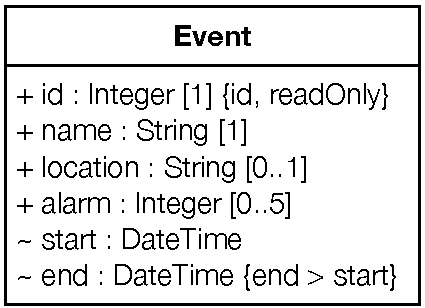
\includegraphics[width=.4\linewidth]{CD-Event.pdf}
	\caption{The Event Class}
	\label{fig:event}
\end{figure}	

\begin{inparaenum}[(A)]
	\item First, declare the Java class and its fields.
	\item Now, declare the class constructor. Remember that some attributes are mandatory and others are not.
	\item Finally, declare the fields' accessors and modifiers (getters and setters). Remember to respect the attribute visibility.
	\item Now, decide how to deal with errors, for instance a start date that is later than the end date. 
\end{inparaenum}
\end{exercise}

\begin{solution}
			There are several ways to deal with errors in Java. In my solution I used assertions, which is a simple solution, but not adapted to public methods. Using runtime exceptions, such as \code{IllegalArgumentException} for the dates and \code{IndexOutOfBoundsException} for multivalued attributes is a more ``java-oriented'' approach. Another interesting approach is the use of AssertJ, which helps developers to specify simple and elegant assertions. Guava, Apache commons, and Lombok are also interesting alternatives to validate parameters.
			
			Alternatives: create our own exceptions, use normal exceptions (not Runtime). Use integers (c-oriented approach.)
%\lstset{language=Java}

\lstinputlisting[language=Java]{./src/main/java/fr/unantes/event/Event.java}

\end{solution}
	
	
\begin{exercise}
	\textbf{Attribute Implementation (Wrapper approach)}
	
Now, use the Wrapper implementation strategy introduced during the lectures to implement the Event class.
	\begin{inparaenum}
		\item For dealing with the multi-valued attribute \code{alarm}, define a wrapper class that is able to check its multiplicity.
		\item Do the same for the mono-valued attributes. Use Java generic types.
	\end{inparaenum}
\end{exercise}
\begin{solution}
	\lstinputlisting[language=Java]{./src/main/java/fr/unantes/event/Event.java}
	\lstinputlisting[language=Java]{./src/main/java/fr/unantes/event/MonovaluedAttribute.java}
	\lstinputlisting[language=Java]{./src/main/java/fr/unantes/event/ReadOnlyMonovaluedAttribute.java}
	\lstinputlisting[language=Java]{./src/main/java/fr/unantes/event/MultivaluedAttribute.java}
\end{solution}


\begin{exercise}
	\textbf{Unidirectional Association Implementation}

Figures~\ref{fig:unidirectional} and~\ref{fig:unique} present two different versions of a unidirectional association between the classes \code{Window} and \code{Field}.
Use Java to implement the classes \code{Window} and \code{Field}, as well as the association between both.

\begin{figure}[htbp]
	\centering
	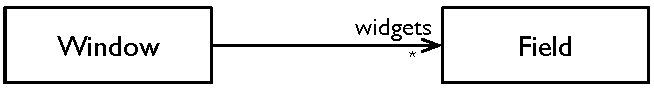
\includegraphics[scale=.8]{CD-WindowFieldUni.pdf}
	\caption{Unidirectional Association}
	\label{fig:unidirectional}
\end{figure}

\begin{figure}[htbp]
	\centering
		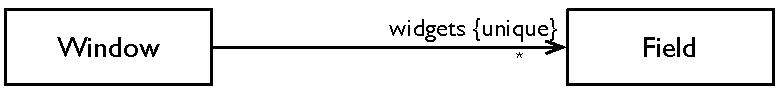
\includegraphics[scale=.8]{CD-WindowFieldUnique.pdf}
	\caption{Unidirectional Unique Association}
	\label{fig:unique}
\end{figure}



\begin{inparaenum}[(A)]
	\item First, for dealing with unidirectional multivalued association roles, define a generic class named \code{Reference} that could be reused by other implementations.
	\item Make your class flexible enough to handle unique et non unique association roles.
	\item Then, declare the Java classes and its fields.
\end{inparaenum}

\end{exercise}

\begin{solution}
		\lstset{language=Java}
		\lstinputlisting{./src/main/java/fr/unantes/unidirectional/Window.java}
		\lstinputlisting{./src/main/java/fr/unantes/unidirectional/Field.java}	
\end{solution}



\begin{exercise}
	\textbf{Bidirectional Association Implementation}

The UML class model presented in Figures~\ref{fig:readOnly} and~\ref{fig:bidirectional}
are similar to the previous ones, except that the association between both classes are bidirectional.

Use Java to implement the classes \code{Window} and \code{Field}, as well as the association between both.
Remember that you must handle the handshake problem.

\begin{figure}[htbp]
	\centering
		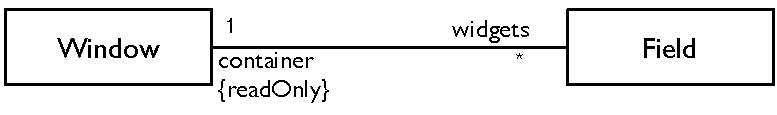
\includegraphics[scale=.8]{CD-WindowFieldReadOnly.pdf}
	\caption{Bidirectional Read-Only Association}
	\label{fig:readOnly}
\end{figure}

\begin{figure}[htbp]
	\centering
		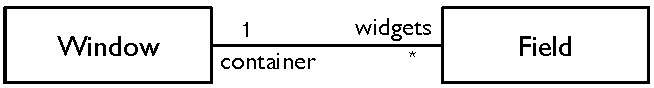
\includegraphics[scale=.8]{CD-WindowField.pdf}
	\caption{Bidirectional Association}
	\label{fig:bidirectional}
\end{figure}	


\begin{inparaenum}[(A)]
	\item First, define a class named \code{ReferenceToWindow} that will handle the mono-valued association role \code{container}, from \code{Field} to \code{Window}. This class must implement the methods \code{get()}, \code{set()}, and \code{unset}.
	\item Then, define a class named \code{ReferenceToField} that will handle the multivalued association role \code{widgets}, from \code{Window} to \code{Field}. This class must implement the methods \code{add()}, \code{remove()}, and \code{contains()}.
	\item Now, add the code needed to handle the handshake. 
	\item Finally, declare the Java classes \code{Window} and \code {Field}, and their fields.
\end{inparaenum}
	
\end{exercise}

\begin{solution}
		\lstset{language=Java}
		\lstinputlisting{./src/main/java/fr/unantes/bidirectional/Window.java}
		\lstinputlisting{./src/main/java/fr/unantes/bidirectional/Field.java}	
\end{solution}

\begin{exercise}
	\textbf{Wrapping Things Up}
	
	Use Java to implement the diagram depicted by Figure~\ref{fig:team}.

	\begin{figure}[htbp]
		\centering
			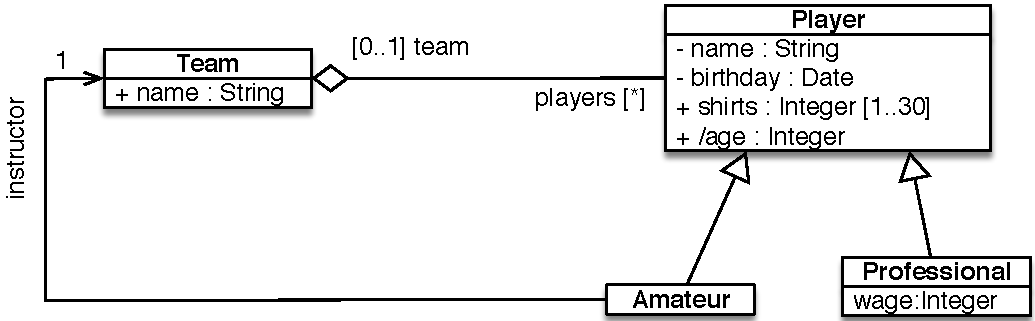
\includegraphics[width=.8\linewidth]{Team}
		\caption{UML Class Diagram\--- Team}
		\label{fig:team}
	\end{figure}
	
\end{exercise}

\chapter{Mapping UML Designs to Code \\ Behavioral Aspects}

\section{Implementing Operations from pre- and post-conditions specifications}

	Consider the class \code{Interval}, illustrated by Figure~\ref{fig:interval}.
	This class has one invariant (Listing~\ref{lst:interval:inv}) and two operations,
	\code{overlapsWith()} (Listing~\ref{lst:overlaps}) and \code{includes()} (Listing~\ref{lst:includes}).

\begin{figure}[htbp]
	\centering
		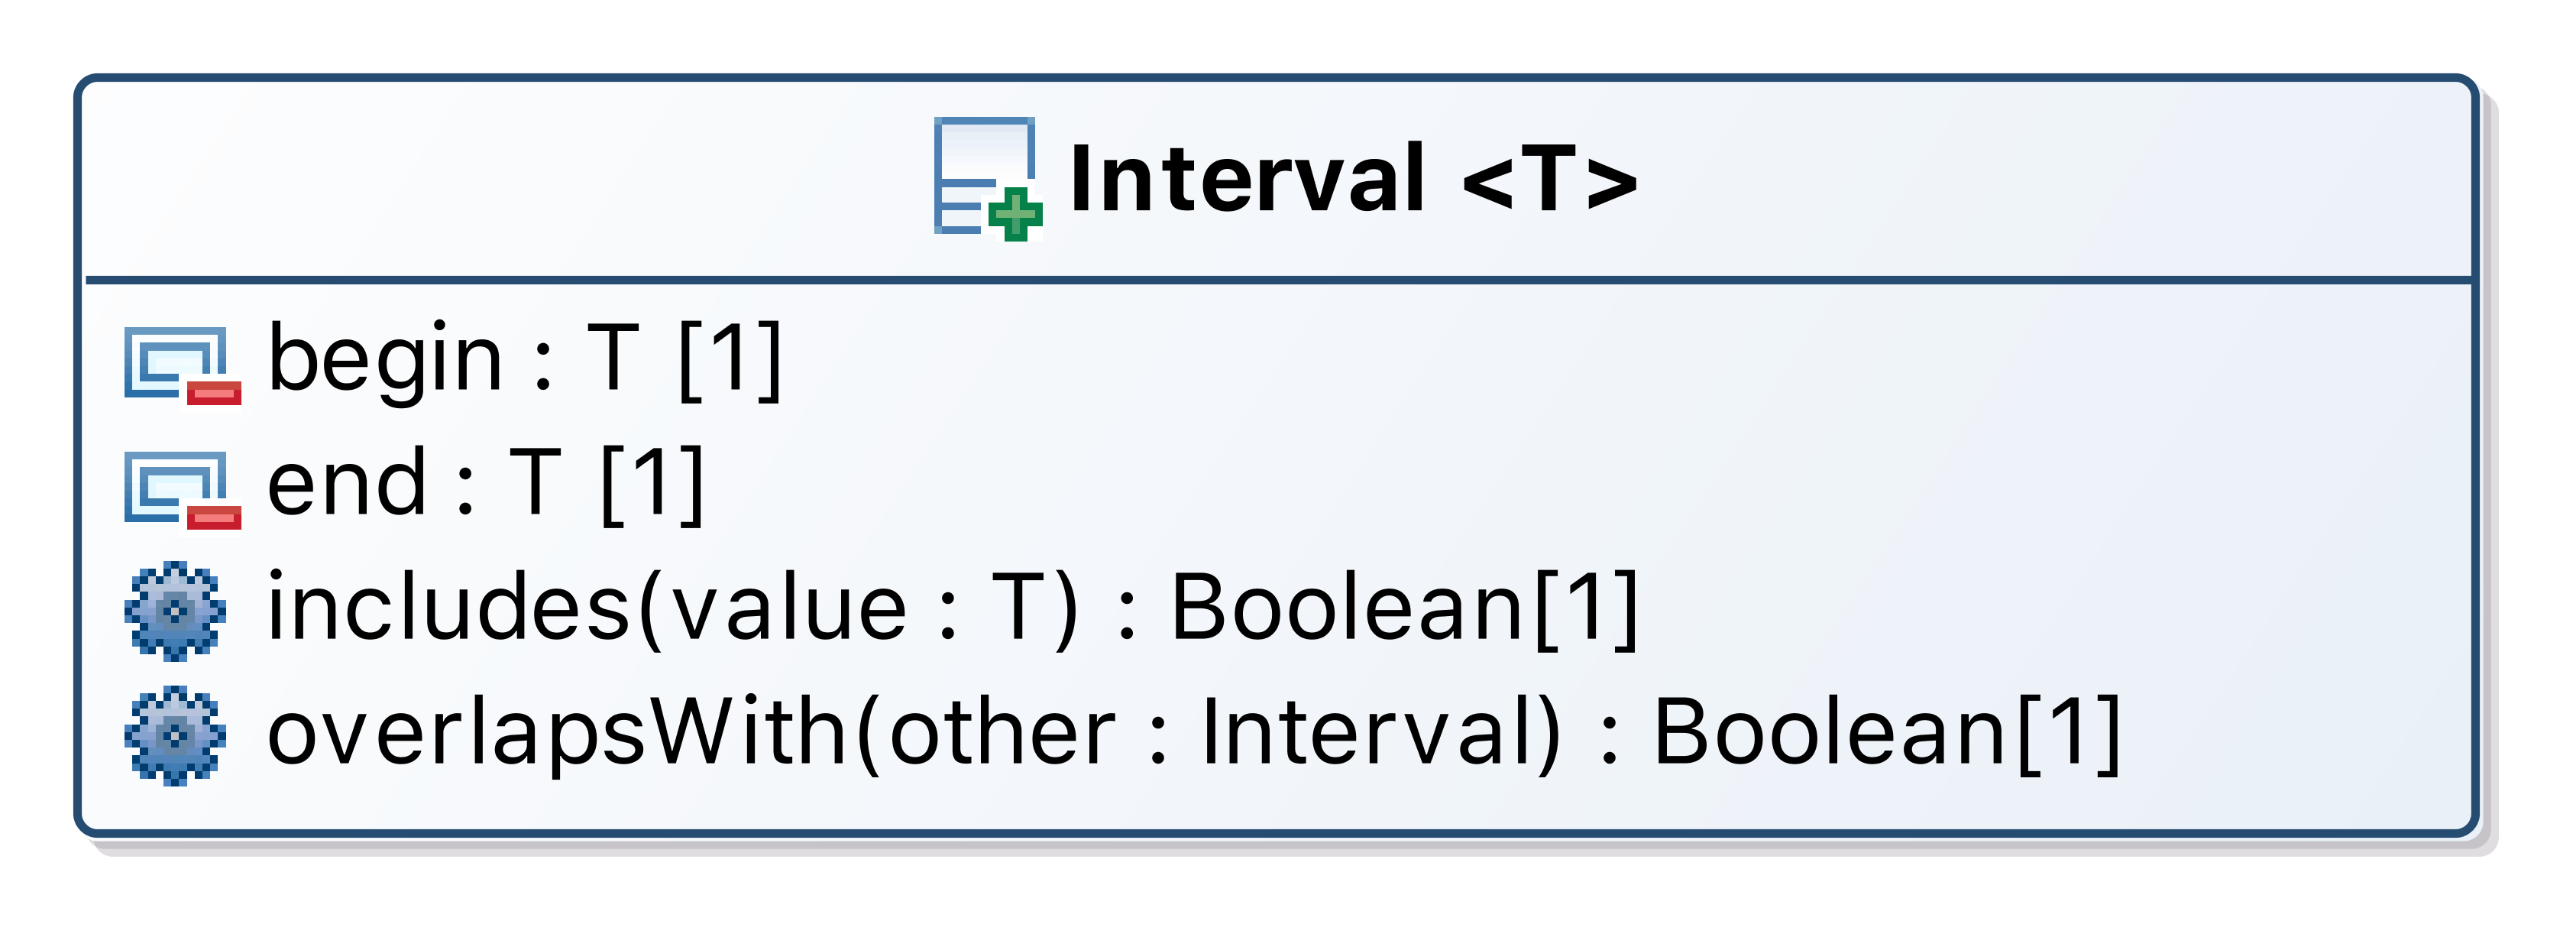
\includegraphics[width=.4\linewidth]{Interval.png}
	\caption{The class «Interval»}
	\label{fig:interval}
\end{figure}


\lstset{caption={Interval invariant},label=lst:interval:inv,float=htbp}
\begin{ocl}
context Interval(T)
inv: self.end > self.begin
\end{ocl}

\lstset{caption={Operation overlapsWith()},label=lst:overlaps,float=htbp}
\begin{ocl}
context Interval(T)::overlapsWith(other : Interval(T)):Boolean
-- This interval overlaps with another if it includes the others begin or end values
-- or if the other contains this interval begin value.
post: result = self.includes(other.begin) or self.includes(other.end) or
			other.includes(self.begin)
\end{ocl}


\lstset{caption={Operation includes()},label=lst:includes,float=htbp}
\begin{ocl}
context Interval(T)::includes(value : T):Boolean
-- This interval includes a value if it is between begin and end.
post: result = value >= begin and value <= end
\end{ocl}


\begin{exercise}
	First, use JUnit to write some unit tests that verify that the class invariant is correctly respected as well as the correction of the tool operations.
\end{exercise}

\begin{solution}
	\lstset{language=Java}
	\lstinputlisting[language=Java]{./src/test/java/fr/unantes/agenda/IntervalTest.java}
\end{solution}

\begin{exercise}
	Second, implement the class «Interval» and its two attributes, without the two operations.
	Propose an approach to ensure that the class invariant will never be violated.
\end{exercise}

\begin{solution}
	Sorry no correction for now, but I guess the invariant can be checked in the constructor and both attributes could be final.
\end{solution}

\begin{exercise}
	 Finally, implement the operations \code{includes()} and \code{overlapsWith()}, respecting the post-conditions specified above.
\end{exercise}

\begin{solution}
	\lstset{language=Java, caption={Class Interval},}
			\lstinputlisting[language=Java]{./src/main/java/fr/unantes/agenda/Interval.java}
\end{solution}

\newpage
\section{Implementing Operations from Activity diagrams}

Consider the classes \code{Event}, \code{SingleEvent} and \code{RecurrentEvent} illustrated by Figure~\ref{fig:recurrent}.
The class \code{Event} has only one operations, \code{conflictsWith()}, whose algorithm is given by Figure~\ref{fig:conflicts}.
The goal of this operation is to check whether two events happen at the same time. 
This is rather simple for single events, but complex for recurrent events.


\begin{figure}[htbp]
	\centering
		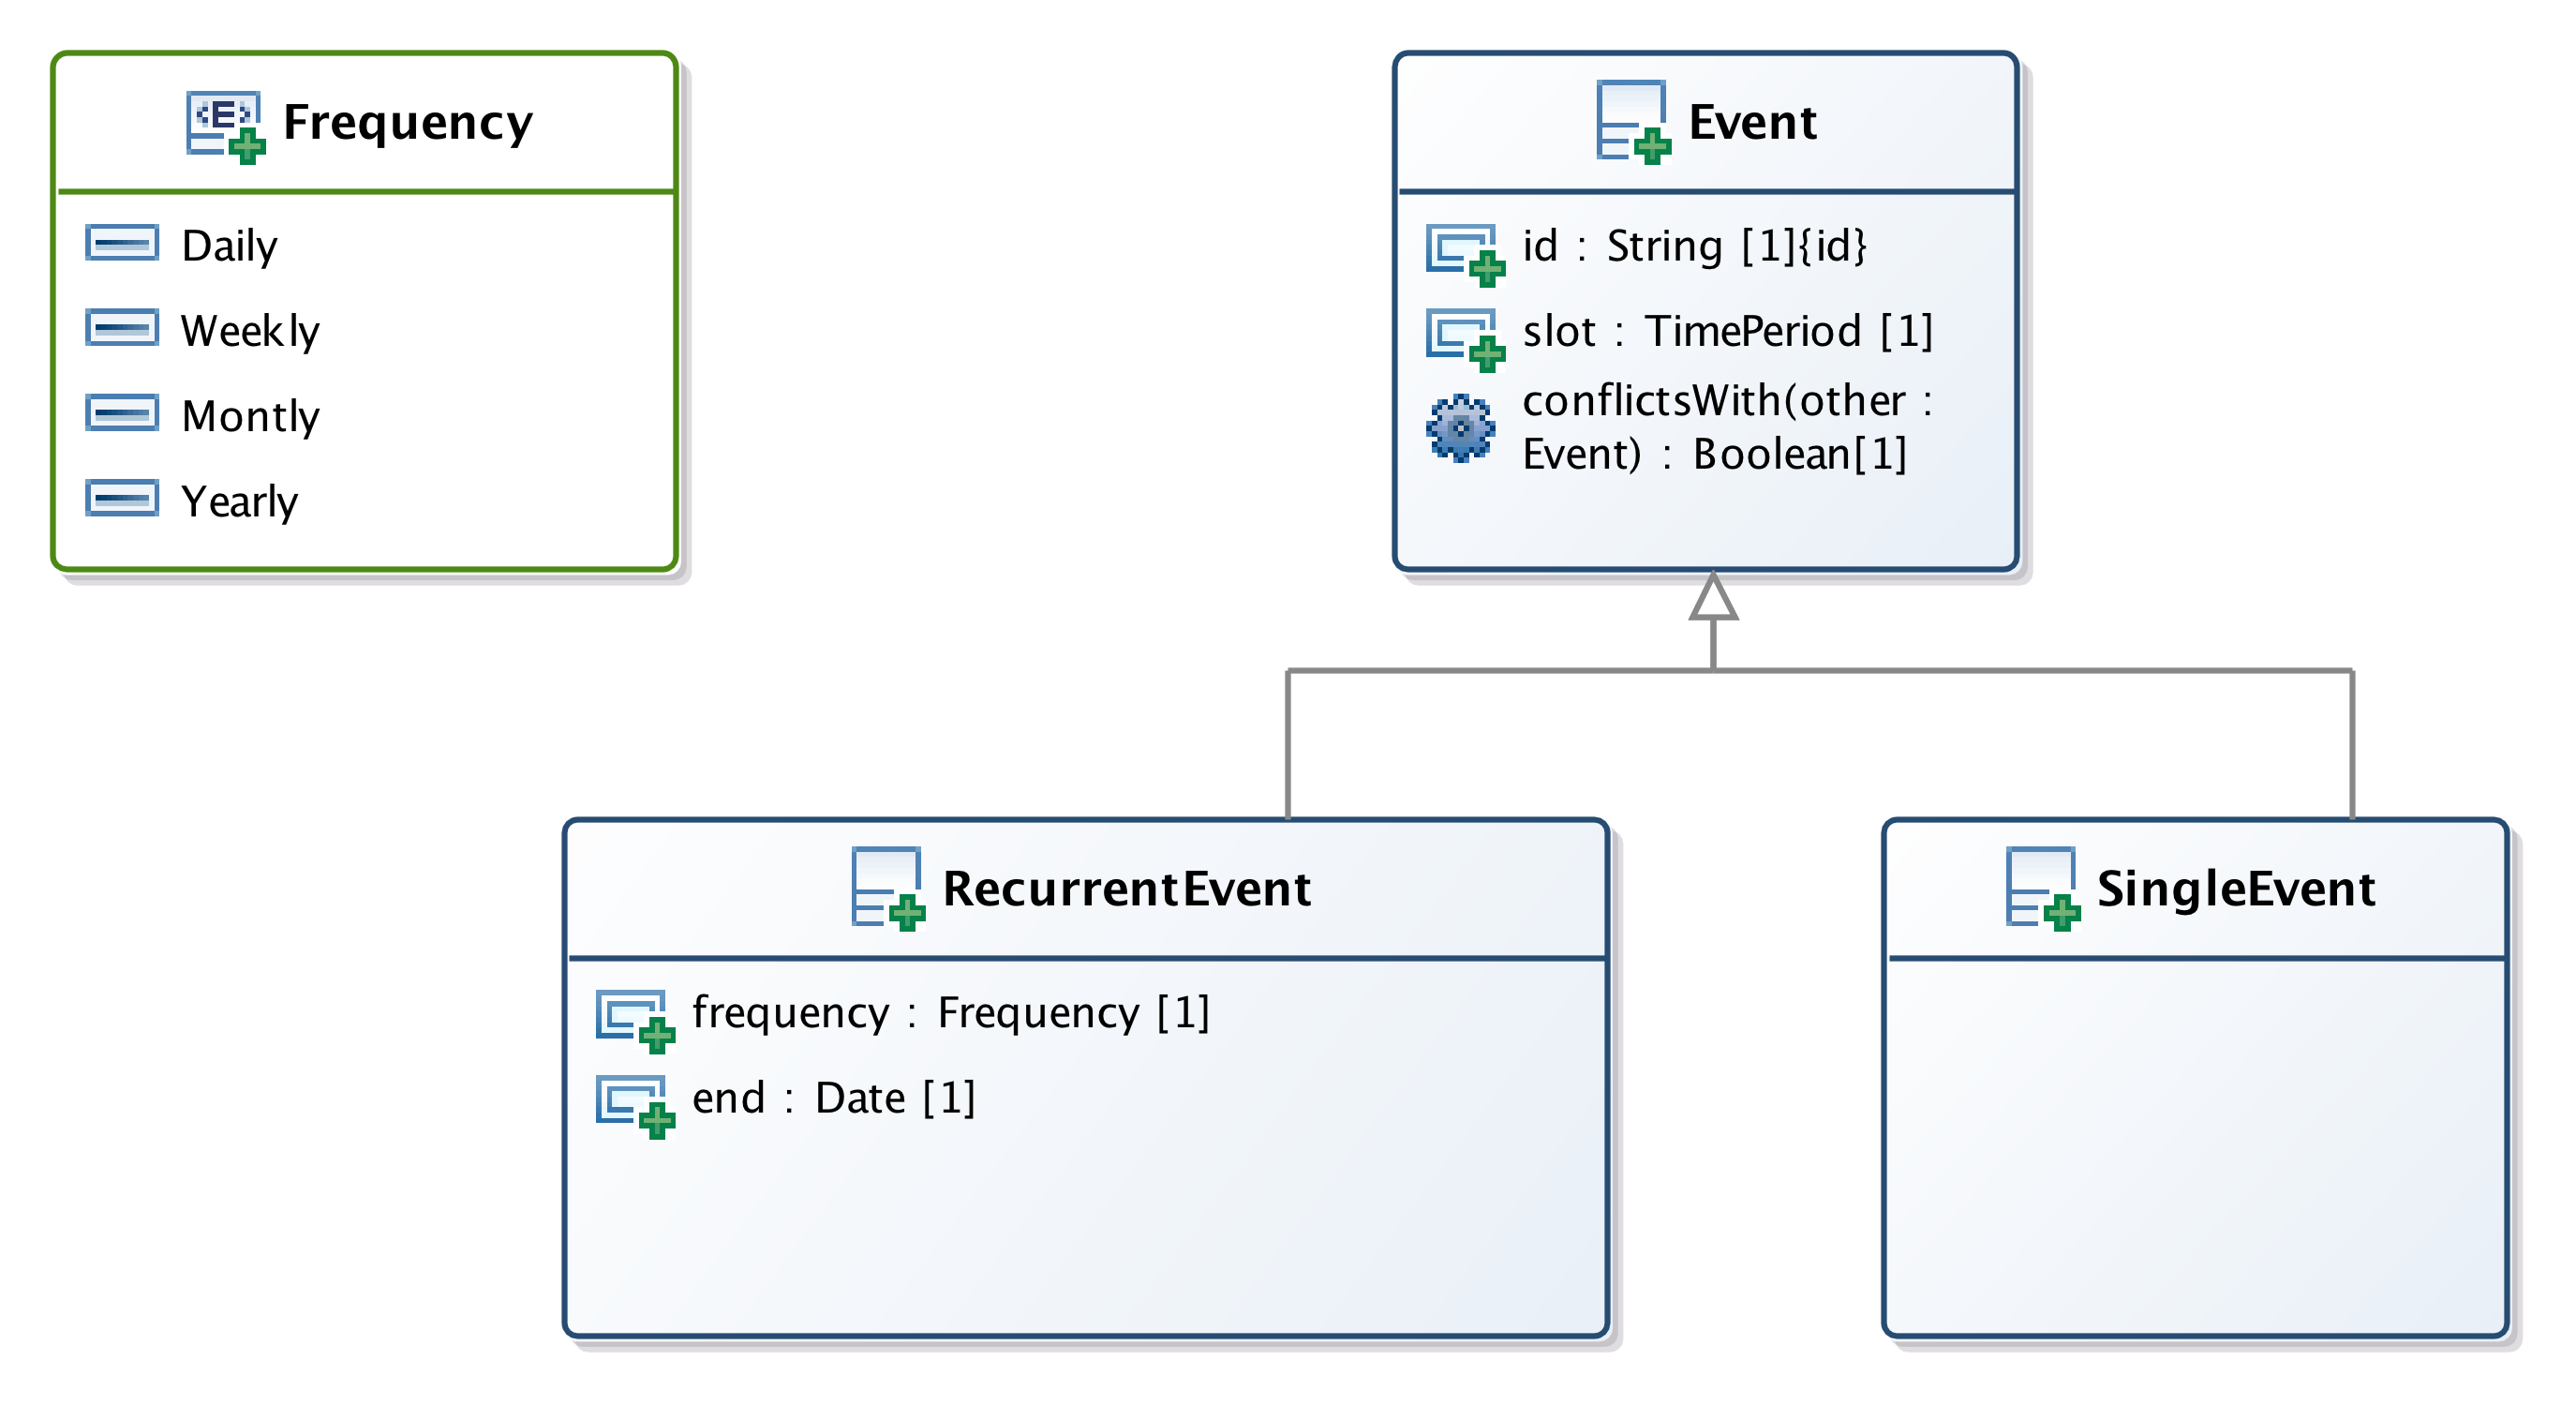
\includegraphics[width=.8\linewidth]{cd-recurrent-event.png}
	\caption{Classes «Event», «SingleEvent», and «RecurrentEvent»}
	\label{fig:recurrent}
\end{figure}


\begin{figure}[htbp]
	\centering
		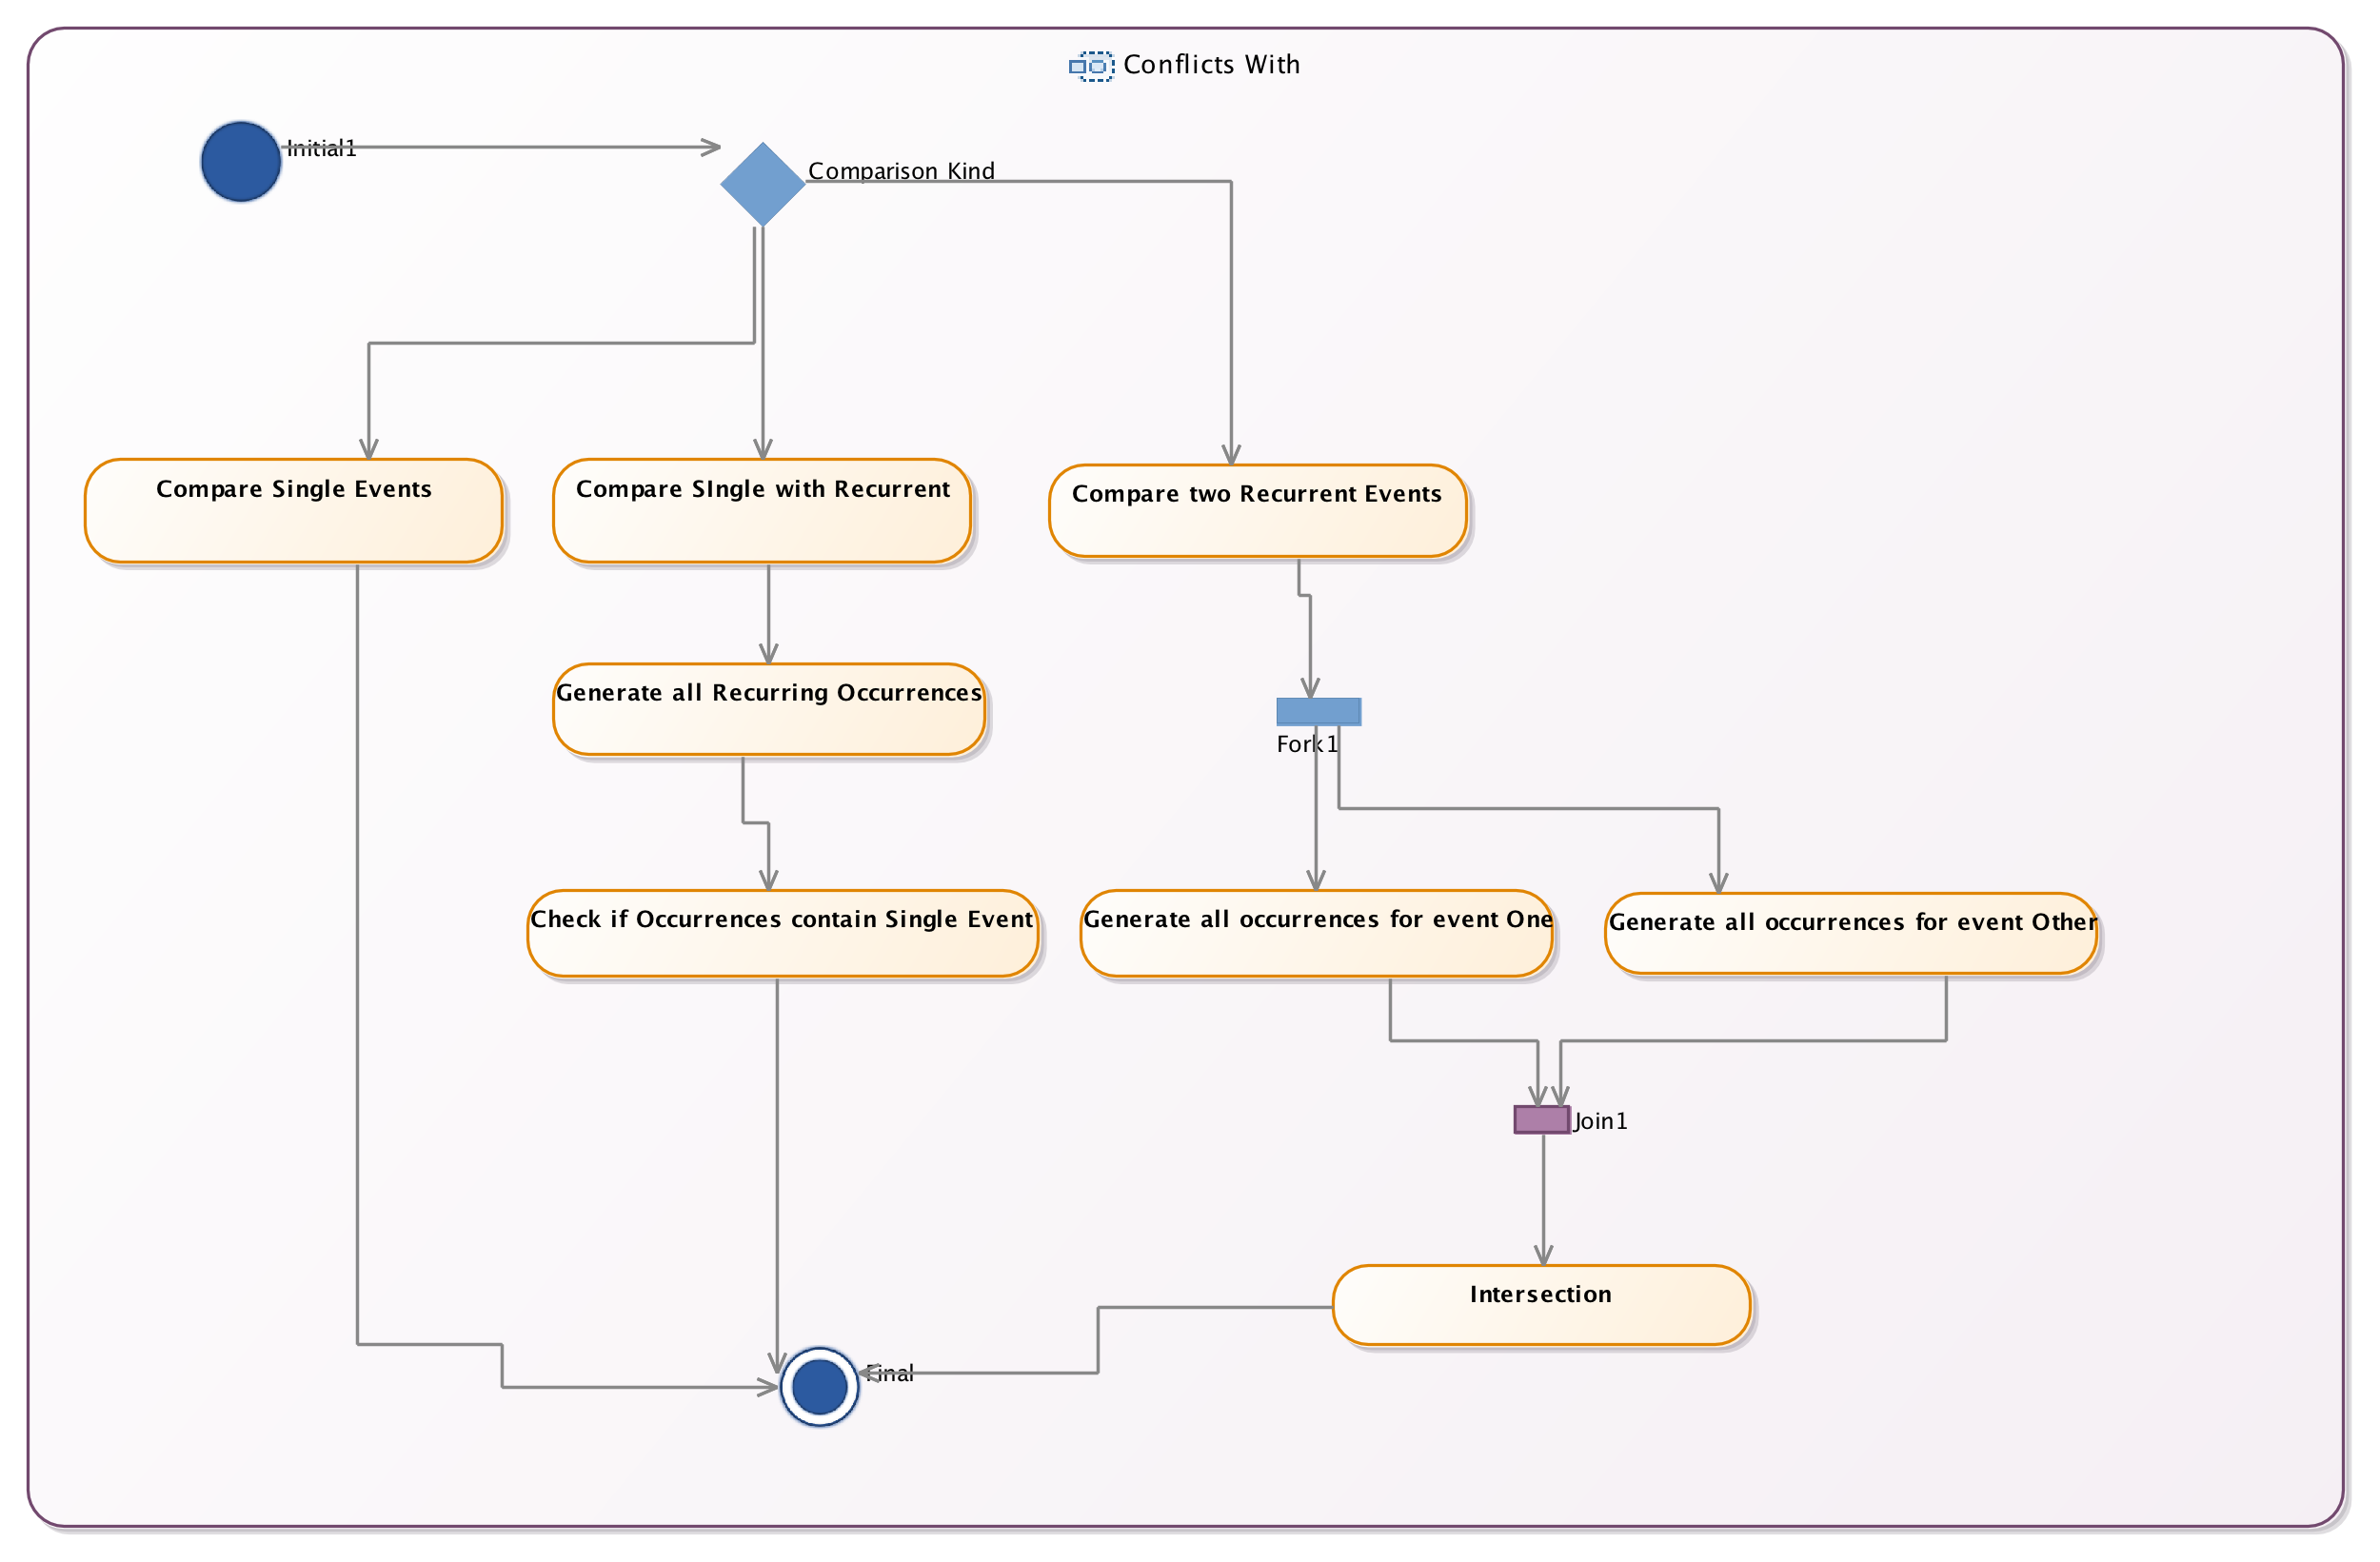
\includegraphics[width=\linewidth]{ad-conflicts.png}
	\caption{Activity Diagram for «conflictsWith» operation}
	\label{fig:conflicts}
\end{figure}


\begin{exercise}
	First, use a «double dispatch» mechanism to choose the correct implementation of the \code{conflictsWith()} operation.
	
	\begin{inparaenum}[(A)]
		\item Add the methods \code{conflictsWithSingleEvent()} and \code{conflictsWithRecurrentEvent()} to the \code{Event} class.
		\item Implement the methods \code{SingleEvent::conflictsWith()} and \code{RecurrentEvent::conflictsWith()} and make them call the correct implementation methods.
	\end{inparaenum}
\end{exercise}

\begin{solution}
\begin{enumerate}
	\item In the implementation I use the \code{java.time} package. It uses date and time without considering time zones.
	\item The code is still incomplete: the intersection method is still Work TODO.
	\item I'm not a big fan of the double dispatch: it makes the superclass depend on subclasses (bad practice).
	
\end{enumerate}
\end{solution}

\begin{exercise}
Add a method named \code{occurrences()} to class \code{RecurrentEvent}.
This method must generate all occurrences of a recurrent event. 
\end{exercise}

\begin{solution}
\lstset{language=Java, caption={Operation conflictsWith()},}
\lstinputlisting{./src/main/java/fr/unantes/agenda/Event.java}
\lstinputlisting{./src/main/java/fr/unantes/agenda/Frequency.java}
\lstinputlisting{./src/main/java/fr/unantes/agenda/AbstractEvent.java}
\lstinputlisting{./src/main/java/fr/unantes/agenda/SingleEvent.java}
\lstinputlisting{./src/main/java/fr/unantes/agenda/RecurrentEvent.java}
\lstinputlisting{./src/main/java/fr/unantes/agenda/TimeSlot.java}
\end{solution}

\begin{exercise}
Finally, implement the 3 \code{conflictsWith()} methods: one that compares 2 single events, one that compares a single event with
a recurrent event, and one that compares two recurrent events.
\end{exercise}

\chapter{Refactoring to Patterns}

\section{Code Simplification}
\subsection{Introduce Compose Method}
The ``Compose Method\footnote{\url{http://c2.com/ppr/wiki/WikiPagesAboutRefactoring/ComposedMethod.html}}'' pattern is about producing methods that efficiently communicate what they do and how they do what they do. 
According to Kent Beck:

\begin{quotation}
	«Divide your program into methods that perform one identifiable task. Keep all of the operations in a method at the same level of abstraction. 
	This will naturally result in programs with many small methods, each a few lines long.»
\end{quotation}

A Composed Method consists of calls to well-named methods that are all at the same level of detail.
Follow the instructions below to simplify the method \code{add()}~\cite{Kerievsky:2004}:

\lstset{language=Java, caption={Class ArrayList}}
\lstinputlisting{./src/main/java/fr/unantes/refactorings/ArrayList.java}

\begin{exercise}
	Invert the ``readonly'' check to a ``Guard Clause''.
\end{exercise}

\begin{solution}
\begin{lstlisting}[caption=cap,label=lst:lab]
    if (readOnly) {
        return;
    }
\end{lstlisting}

\end{solution}

\begin{exercise}
	Apply the ``Extract Method'' operation to lines 19-20 and create the method \code{void addElement(object)}.
\end{exercise}

\begin{exercise}
	Apply the ``Extract Constant'' operation to replace the magic number ``10 '' and introduce an ``Explaining Variable'' called \code{GROWTH\_INCREMENT}.
\end{exercise}

\begin{exercise}
	Apply the ``Inline variable'' operation to \code{newSize} and then apply the ``Extract Method'' operation again to the code that checks whether the element array is at its capacity and needs to grow, and create the method \code{atCapacity()}.
\end{exercise}

\begin{exercise}
	Finally, apply the ``Extract Method'' operation to the code that grows the size of the \code{elements} array, creating the \code{grow()} method.
\end{exercise}

\begin{solution}
	\lstset{language=Java, caption={Class ArrayList after Refactoring}}
	\lstinputlisting{./src/main/java/fr/unantes/refactorings/ArrayListRefactored.java}
\end{solution}

\newpage

\subsection{Replace Conditional Logic with Strategy}

The  Strategy pattern defines a family of algorithms, encapsulates each algorithm, and make them interchangeable, letting the algorithm vary independently from clients that use it.
We can apply this pattern to classes where several methods have similar structure: a sequence of similar conditions.
For instance, let us consider the \code{Loan} class\footnote{\url{http://www.informit.com/articles/article.aspx?p=1398607&seqNum=2}}, from Joshua Kerievsky's book~\cite{Kerievsky:2004}, presented in Listing~\ref{lst:loan}.

\lstset{caption=The Loan Class,label=lst:loan,float=htbp}
\lstinputlisting{./src/main/java/fr/unantes/refactorings/Loan.java}

This class deals with calculating capital for three different kinds of bank loans: 

\begin{description}
	\item [Term loan]: a loan from a bank for a specific amount that has a specified repayment schedule and a fixed or floating interest rate. 
	\item [Revolver]: a credit that is automatically renewed as debts are paid off; and
	\item [Advised line]: a credit that a financial institution approves and maintains for a customer.
\end{description}

Much of the logic of methods \code{capital()} and \code{duration()} deals with figuring out whether the loan is a term loan, a revolver, or an advised line. 
For example, a null expiry date and a non-null maturity date indicate a term loan. 
A null maturity and a non-null expiry date indicate a revolver loan.

In this exercise, we will use the Strategy pattern to simplify the calculation of the loan's capital.
	

\begin{exercise}
	First, create a class called \code{CapitalStrategy} and add a method called \code{capital()}, with an empty body. 
\end{exercise}
\begin{solution}
\begin{lstlisting}[caption=cap,label=lst:lab]
public class CapitalStrategy {
    public double capital(Loan loan) {
        return 0.0;
    }
}
\end{lstlisting}
\end{solution}

\begin{exercise}
Now, apply the ``Move Method'' refactoring operation to move the \code{capital()} method to class \code{CapitalStrategy}.  This involves:

\begin{enumerate}
	\item Changing the visibility of some private methods: \code{getUnusedPercentage()}, \code{outstandingRiskAmount()}, \code{riskFactor()}, \code{unusedRiskAmount()}, and \code{unusedRiskFactor()}.
	\item Encapsulating fields \code{commitment}, \code{expiry}, \code{maturity}, \code{riskRating}, \code{today}, \code{start}, and \code{payments}.
	\item Creating a simple version of method \code{capital()} on class \code{Loan}, which delegates to an instance of \code{CapitalStrategy}.
	\item Moving the method and replacing all references to \code{this} by \code{loan}.
\end{enumerate}

\end{exercise}
\begin{solution}
	\begin{itemize}
		\item Maybe we should remember that "protected" methods are accessible from classes belonging to the same package.
	\end{itemize}
	
	
\begin{lstlisting}[caption=cap,label=lst:label]
public class LoanRefactored {
    // (...)

    public double capital() {
        return new CapitalStrategy().capital(this);
    }
    // (...)
    protected double riskFactor() {
        return RiskFactor.getFactors().forRating(riskRating);
    }

    protected double unusedRiskFactor() {
        return UnusedRiskFactors.getFactors().forRating(riskRating);
    }

    protected double getUnusedPercentage() {
        return 0.0;
    }

    protected Date getMaturity() {
        return maturity;
    }

    protected Date getExpiry() {
        return expiry;
    }

    protected double getCommitment() {
        return commitment;
    }

    protected List<Payment> getPayments() {
        return payments;
    }
}

public class CapitalStrategy {
    public double capital(LoanRefactored loan) {
        if (loan.getExpiry() == null && loan.getMaturity() != null)
            return loan.getCommitment() * loan.duration() * loan.riskFactor();
        if (loan.getExpiry() != null && loan.getMaturity() == null) {
            if (loan.getUnusedPercentage() != 1.0)
                return loan.getCommitment() *loan.getUnusedPercentage() * loan.duration() * loan.riskFactor();
            else
                return (loan.outstandingRiskAmount() * loan.duration() * loan.riskFactor())
                        + (loan.unusedRiskAmount() * loan.duration() * loan.unusedRiskFactor());
        }
        return 0.0;
    }
}
\end{lstlisting}
\end{solution}

\begin{exercise}
	Apply the ``Move Method'' refactoring operation again to move the \code{duration()} method to class \code{CapitalStrategy}. 
\end{exercise}
\begin{solution}
\begin{lstlisting}[caption={duration() method},label=lst:lab]
    public double duration(LoanRefactored loan) {
        if (loan.getExpiry() == null && loan.getMaturity() != null)
            return this.weightedAverageDuration(loan);
        else if (loan.getExpiry() != null && loan.getMaturity() == null)
            return loan.strategy.yearsTo(loan.getExpiry(), loan);
        return 0.0;
    }
\end{lstlisting}
\end{solution}

\begin{exercise}
	Since some methods, such as \code{duration()}, \code{weightedAverageDuration()}, \code{yearsTo()},  \code{riskFactor()} and \code{unusedRiskFactor()} are only used by method \code{capital()}, we can move them to class \code{CapitalStrategy} as well.
	The two constants, \code{MILLIS\_PER\_DAY} and \code{DAYS\_PER\_YEAR} can also be moved to class  \code{CapitalStrategy}.
\end{exercise}
\begin{solution}
	\begin{itemize}
		\item After these refactorings, the code should be: 
	\end{itemize}
	\lstset{caption={The LoanRefactored Class},label=lst:loan:refactored,float=htbp}
	\lstinputlisting{./src/main/java/fr/unantes/refactorings/LoanRefactored.java}
	\lstset{caption=The CapitalStrategy Class,label=lst:capital:strategy,float=htbp}
	\lstinputlisting{./src/main/java/fr/unantes/refactorings/CapitalStrategy.java}
\end{solution}

\begin{exercise}
	Finally, apply the ``Replace Conditional with Polymorphism '' refactoring operation on method \code{capital()} method. 
	First, create a subclass named \code{CapitalStrategyTermLoan} for the capital calculation for a term loan.
	Then, move and adapt methods \code{capital()}, \code{duration}, and \code{weightedAverageDuration} to the subclass.
\end{exercise}

\begin{solution}
	\begin{lstlisting}[caption=cap,label=lst:lab]
public class CapitalStrategyTermLoan extends CapitalStrategy {
   public double capital(Loan loan) {
      return loan.getCommitment() * duration(loan) * riskFactorFor(loan);
   }

   public double duration(Loan loan) {
      return weightedAverageDuration(loan);
   }

   private double weightedAverageDuration(Loan loan) {
      double duration = 0.0;
      double weightedAverage = 0.0;
      double sumOfPayments = 0.0;
      Iterator loanPayments = loan.getPayments().iterator();
      while (loanPayments.hasNext()) {
         Payment payment = (Payment)loanPayments.next();
         sumOfPayments += payment.amount();
         weightedAverage += yearsTo(payment.date(), loan) * payment.amount();
      }
      if (loan.getCommitment() != 0.0)
         duration = weightedAverage / sumOfPayments;
      return duration;
   }		
	\end{lstlisting}

In the end, class \code{CapitalStrategy} is abstract:


	\lstset{caption={The CapitalStrategy Class - Final version},label=lst:capital:strategy,float=htbp}
	\lstinputlisting{./src/main/java/fr/unantes/refactorings/CapitalStrategyRefactored.java}

\end{solution}

\newpage

\section{Chain Constructors}

Classes may have several constructors: this is normal, as there may be different ways to instantiate objects of a same class.
However, when there is duplicated code across two or more contacts, maintenance problems arise. 

Consider the three constructors of class \code{Loan}~\cite{Kerievsky:2004}, presented in Listing~\ref{lst:loan:constructors}, which have duplicated code.
We will use the refactoring operation named ``Chain Constructors'', whose goal is to remove duplication in constructors by making them call each other.

First, we analyze these constructors to find out which one is the ``catch-all constructor'', the one that handles all of the construction details.
It seems that it should be constructor 3, since making constructors 1 and 2 call 3 can be achieved with a minimum amount of work.

\begin{lstlisting}[caption={Constructors for class \code{Loan}},label=lst:loan:constructors,float=htbp,frame=tb]
public Loan(float notional, float outstanding, int rating, Date expiry) {
   this.strategy = new TermROC();
   this.notional = notional;
   this.outstanding = outstanding;
   this.rating = rating;
   this.expiry = expiry;
}

public Loan(float notional, float outstanding, int rating, Date expiry, Date maturity) {
   this.strategy = new RevolvingTermROC();
   this.notional = notional;
   this.outstanding = outstanding;
   this.rating = rating;
   this.expiry = expiry;
   this.maturity = maturity;
}

public Loan(CapitalStrategy strategy, float notional, float outstanding, int rating, Date expiry, Date maturity) {
   this.strategy = strategy;
   this.notional = notional;
   this.outstanding = outstanding;
   this.rating = rating;
   this.expiry = expiry;
   this.maturity = maturity;
}
\end{lstlisting}



\begin{exercise}
Change constructor 1 to make it call constructor 3.
\end{exercise}

\lstset{caption={}}
\begin{solution}
\begin{java}
public Loan(float notional, float outstanding, int rating, Date expiry) {
    this(new TermROC(), notional, outstanding, rating, expiry, null);
}	
\end{java}
\end{solution}


\begin{exercise}
Now, change constructor 2 to make it also call constructor 3.
\end{exercise}

\begin{solution}
\begin{java}
public Loan(float notional, float outstanding, int rating, Date expiry, Date maturity) {
    this(new RevolvingTermROC(), notional, outstanding, rating, expiry, maturity);
}	
\end{java}
\end{solution}


\section{Replace Constructors with Creation Methods}
The goal of the ``Replace Constructors with Creation Methods'' refactoring operation is to 
replace constructors with intention-revealing creation methods that return object instances.

Creation methods have at least two advantages, that cannot be achieved in Java. 
First, they can have different names and thus communicate intention efficiently.
Second, creation methods can have the same number of parameters.

We will apply this refactoring to improve the constructions of class \code{Loan}.
Consider another version of class \code{Loan}, presented in Listing~\ref{lst:load:constructors:bis}.

\begin{lstlisting}[caption={Cascade Constructors for class \code{Loan}},label=lst:load:constructors:bis,float=htbp]
public class Loan {

    double commitment;
    double outstanding;
    int riskRating;
    Date maturity;
    Date expiry;
    CapitalStrategy capitalStrategy;

    public Loan(double commitment, int riskRating, Date maturity) {
        this(commitment, 0.00, riskRating, maturity, null);
    }

    public Loan(double commitment, int riskRating, Date maturity, Date expiry) {
       this(commitment, 0.00, riskRating, maturity, expiry);
    }

    public Loan(double commitment, double outstanding, int riskRating, Date maturity, Date expiry) {
        this(null, commitment, outstanding, riskRating, maturity, expiry);
    }

    public Loan(CapitalStrategy capitalStrategy, double commitment, int riskRating, Date maturity, Date expiry) {
        this(capitalStrategy, commitment, 0.00, riskRating, maturity, expiry);
    }

    public Loan(CapitalStrategy capitalStrategy, double commitment, double outstanding, int riskRating, Date maturity,
            Date expiry) {
        this.commitment = commitment;
        this.outstanding = outstanding;
        this.riskRating = riskRating;
        this.maturity = maturity;
        this.expiry = expiry;
        this.capitalStrategy = capitalStrategy;

        if (capitalStrategy == null) {
            if (expiry == null)
                this.capitalStrategy = new CapitalStrategyTermLoan();
            else if (maturity == null)
                this.capitalStrategy = new CapitalStrategyRevolver();
            else
                this.capitalStrategy = new CapitalStrategyRCTL();
        }
    }
}
\end{lstlisting}


To apply this refactoring, we need to find a code that calls one of these constructors. For instance, in a test case:
\begin{java}
public class CapitalCalculationTests...
   public void testTermLoanNoPayments() {
      //...
      Loan termLoan = new Loan(commitment, riskRating, maturity);
      //...
   }
\end{java}

\begin{exercise}
	First, apply the ``Extract Method'' refactoring on that constructor call to produce a public, static method called \code{createTermLoan()}.
\end{exercise}
\begin{solution}
\begin{java}
public class CapitalCalculationTests{
	public void testTermLoanNoPayments() {
      //...
      Loan termLoan = createTermLoan(commitment, riskRating, maturity);
      //...
   }
   
	public static Loan createTermLoan(double commitment, int riskRating, Date maturity) {
		return new Loan(commitment, riskRating, maturity);
	}
}
\end{java}	
\end{solution}

\begin{exercise}
	Next, apply the ``Move Method'' refactoring on the creation method, \code{createTermLoan()}, to move it to \code{Loan}. 
\end{exercise}
\begin{solution}
\begin{java}
public class Loan {
    // ...
    public static Loan createTermLoan(double commitment, int riskRating, Date maturity) {
        return new Loan(commitment, riskRating, maturity);
    }
}

public class CapitalCalculationTest {
    //...
    public void testTermLoanNoPayments() {
        // ...
        Loan termLoan = Loan.createTermLoan(commitment, riskRating, maturity);
        //...
   }
}
\end{java}
\end{solution}

\begin{exercise}
After doing that, we will need to find all callers of the constructor and update them to call \code{createTermLoan()}.
Since now the \code{createTermLoan()} method is now the only caller on the constructor, we can apply the ``Inline Method''
refactoring to this constructor.
\end{exercise}

\begin{solution}
\begin{java}
public static Loan createTermLoan(double commitment, int riskRating, Date maturity) {
    return new Loan(commitment, 0.00, riskRating, maturity, null);
}        
\end{java}
\end{solution}

\begin{exercise}
    Repeat the same procedure  to the other constructors, to create additional creation methods on class \code{Loan}.
\end{exercise}
\begin{solution}
\begin{java}
public static Loan newRevolver(double commitment, Date start, Date expiry, int riskRating) {
    return new Loan(commitment, 0, start, expiry, null, riskRating, new CapitalStrategyRevolver());
}

public static Loan newAdvisedLine(double commitment, Date start, Date expiry, int riskRating) {
    if (riskRating > 3) return null;
    Loan advisedLine = new Loan(commitment, 0, start, expiry, null, riskRating, new CapitalStrategyAdvisedLine());
      advisedLine.setUnusedPercentage(0.1);
      return advisedLine;
}
\end{java}
\end{solution}

\begin{exercise}
    Last step, since the constructors are only used by creation methods, they can become private.
\end{exercise}


\bibliographystyle{abbrv}
\bibliography{references}
\end{document}


